\chapter{Background}
In questo capitolo vengono descritte le basi teoriche necessarie per introdurre il lavo
ro svolto. In particolare i concetti su cui si basano GAMMA e Olivander, i due algoritmi usati in questo caso di studio.

\section{File Windows PE}
Il formato Portable Executable (PE) costituisce lo standard de facto per i file eseguibili, il codice oggetto,
le librerie a collegamento dinamico (DLL) e altri file immagine utilizzati nelle versioni a 32 e 64 bit dei sistemi 
operativi Microsoft Windows.\cite{PeFormatDocs}


Lo standard è condiviso sia per i file eseguibili (detti `image`) e gli object-file;per lo scopo della tesi sono di interesse solo i file eseguibili

\subsection{Struttura generale}
Un file PE è organizzato in una struttura gerarchica composta da header, tabelle di dati e sezioni. 
La struttura può essere suddivisa nei seguenti componenti principali\cite{PeFormatDocs}:

\begin{itemize}
    \item \textbf{DOS Header e DOS Stub}: per compatibilità con sistemi MS-DOS legacy, viene inserito un eseguibile segnaposto (stub) per i sistemi DOS, che stampa a schermo la stringa \texttt{This program cannot be run in DOS mode}, e un puntatore all'header PE
    \item \textbf{PE HEADER}: firma (signature) del file PE (\texttt{PE\textbackslash0\textbackslash0}, le lettere ``P'' ed ``E'' seguite da due null-byte) e la intestazione del file (IMAGE\_FILE\_HEADER) che contiene informazioni sulla compilazione
    \item \textbf{COFF File Header}: informazioni sulla architettura target, numero di sezioni e caratteristiche generali
    \item \textbf{Optional Header}: metadati essenziali per il caricamento, per esempio se l'architettura target è a 32 o 64bit, versione, Checksum etc..
    \item \textbf{Section Table}: array di descrittori delle sezioni
    \item \textbf{Sections}: il contenuto effettivo del programma organizzato in sezioni
\end{itemize}

\begin{figure}[ht]
    \centering
    \includegraphics[width=0.8\textwidth]{images/pe-structure.png}
    \caption{Struttura generale di un file PE: dal header DOS alle sezioni\cite{MZRSTpeStructure}}
    \label{fig:pe-structure}
\end{figure}

\subsubsection{Le sezioni in un file PE}
Contenute dopo tutti gli header di un file PE,le sezioni rappresentano i blocchi funzionali in cui è suddiviso il contenuto di un file PE, e ne occupano il resto del contenuto.Ogni sezione 
è descritta da una entry nella Section Table (struttura \texttt{IMAGE\_SECTION\_HEADER}) che specifica le sue proprietà principali, riassunte nella tabella seguente:

\begin{table}[H]
\caption{Descrittore di una sezione}
\label{tab:section-header}
\centering
\begin{tabular}{@{}p{0.25\textwidth}p{0.70\textwidth}@{}}
\toprule
\textbf{Campo} & \textbf{Descrizione} \\
\midrule
\textbf{Name} & Nome della sezione (fino a 8 caratteri). \\
\textbf{VirtualSize} & Dimensione della sezione quando caricata in memoria. \\
\textbf{VirtualAddress} & Indirizzo relativo della sezione in memoria (RVA). \\
\textbf{SizeOfRawData} & Dimensione della sezione su disco (allineata a \texttt{FileAlignment}). \\
\textbf{PointerToRawData} & Offset fisico della sezione nel file. \\
\textbf{Characteristics} & Flag che definiscono gli attributi: leggibile, scrivibile, eseguibile, contenuto codice/dati, condivisibile, eliminabile dalla memoria, ecc. \\
\bottomrule
\end{tabular}
\end{table}

Le sezioni consistono di semplici blocchi di byte. Le sezioni standard più comuni sono riassunte nella seguente tabella:

\begin{table}[H]
\caption{Sezioni standard più comuni in un file PE}
\label{tab:pe-sections}
\centering
\begin{tabular}{@{}p{0.15\textwidth}p{0.78\textwidth}@{}}
\toprule
\textbf{Nome} & \textbf{Descrizione} \\
\midrule
\texttt{.text} & Contiene il codice eseguibile del programma. Questa sezione è tipicamente marcata come eseguibile e di sola lettura. È la sezione principale dove risiede la logica dell'applicazione. \\
\texttt{.data} & Contiene dati inizializzati e scrivibili. Include variabili globali e statiche con valori iniziali definiti nel codice sorgente. \\
\texttt{.rdata} & Contiene dati di sola lettura, come costanti stringa, tabelle di virtual function (vtable) e la Import Address Table (IAT). \\
\texttt{.bss} & Contiene dati non inizializzati. Occupa spazio in memoria ma non nel file su disco, poiché verrà azzerata al caricamento. \\
\texttt{.rsrc} & Contiene le risorse del programma: icone, bitmap, stringhe localizzate, menu, dialog box e altri elementi dell'interfaccia utente. \\
\texttt{.reloc} & Contiene informazioni di rilocazione necessarie per l'Address Space Layout Randomization (ASLR). Permette al loader di modificare gli indirizzi quando il programma non può essere caricato al suo indirizzo base preferito. \\
\texttt{.edata} & Contiene la Export Directory Table per DLL che esportano funzioni utilizzabili da altri moduli. \\
\texttt{.idata} & Contiene la Import Directory Table con informazioni sulle funzioni importate da altre DLL. \\
\texttt{.pdata} & Contiene informazioni per la gestione delle eccezioni. \\
\texttt{.tls} & Contiene dati per variabili thread-specific. (Thread Local Storage) \\
\bottomrule
\end{tabular}
\end{table}

\paragraph{Sezioni personalizzate}
Oltre alle sezioni standard, un file PE può contenere sezioni personalizzate con nomi arbitrari. 
Il formato è estremamente flessibile: le sezioni non devono seguire un ordine particolare, 
possono avere dimensioni diverse su disco e in memoria, e possono contenere spazi non utilizzati.

\begin{figure}[ht]
    \centering
    \includegraphics[width=0.8\textwidth]{images/winInternal.png}
    \caption{Sezioni di un file PE, viste da winInternal}
    \label{fig:winInternal}
\end{figure}

% Questa flessibilità rende le sezioni PE un obiettivo privilegiato per tecniche di evasione e 
% offuscamento. Gli attaccanti possono:

% \begin{itemize}
%     \item Aggiungere sezioni personalizzate con payload malevoli
%     \item Modificare i permessi delle sezioni esistenti
%     \item Nascondere dati negli spazi non utilizzati tra le sezioni
%     \item Manipolare i descrittori mantenendo la funzionalità del file
%     \item Sfruttare discrepanze tra VirtualSize e SizeOfRawData
%     \item Alterare l'entry point per eseguire codice da sezioni non standard
% \end{itemize}

% Queste caratteristiche rendono il formato PE particolarmente interessante per gli attacchi 
% adversarial che mirano a evadere i sistemi di rilevamento basati su machine learning, 
% come verrà approfondito nei capitoli successivi.

\section{LIEF per l'analisi statica dei file windows PE}
\label{LIEF_data}
LIEF (Library to Instrument Executable Formats) è una libreria open-source ampiamente utilizzata 
per la manipolazione e l'analisi statica di file binari, con particolare supporto per il formato 
Windows PE\cite{LIEF}. Sviluppata originariamente da Quarkslab, LIEF fornisce un'interfaccia 
unificata per lavorare con diversi formati eseguibili (PE, ELF, Mach-O). 

LIEF è stato usato per estrarre 2381 caratteristiche~(feature) del dataset EMBER~\cite{2018arXiv180404637A}
Dal suo rilascio, il dataset originale EMBER  è stato citato più di 600 volte,da più di  350  istituzioni citanti uniche  in 6 continenti~\cite{Joyce_2025}.\linebreak
Le caratteristiche analizzate si possono dividere in 9 gruppi: \label{feature_set}

\subsection{Informazioni dal formato PE}
\paragraph{Informazioni generali sul file} (10 feature) in questo gruppo sono incluse le caratteristiche recuperabili dal intestazione del file PE, quindi la grandezza del eseguibile una volta mappato su memoria virtuale, il numero di funzioni importate ed esportate, presenza di determinate sezioni,risorse, etc ..
\paragraph{Informazioni dal COFF/Optional Header} (62 feature) in questo gruppo sono incluse le caratteristiche recuperabili dall'header COFF e dall'header opzionale, dato che le informazioni contenute in questi header sono principalmente in formato stringa o lista di stringhe vengono sintetizzati utilizzando la tecnica del feature hashing\cite{hashTrick} (chiamato anche hash-trick) con 10 bin allocati per ciascun noise-vector.
\paragraph{Informazioni sulle funzioni importate} (1280 feature) in questo gruppo sono incluse le caratteristiche recuperabili analizzando la IAT raggruppate per libreria di origine. anche qui le stringhe \texttt{funzione:libreria} sono compresse usando l'hashTrick (256 bins per le librerie, 1024 per le funzioni).
\paragraph{Informazioni sulle funzioni esportate} (128 feature) in questo gruppo sono incluse le caratteristiche recuperabili analizzando la EAT, riassunte tramite hashTrick in 128 bins
\paragraph{Informazioni sulle sezioni} (255 feature) descrive i dati registrati nell'header delle sezioni (es. nome, dimensione, entropia, VirtualSize), con particolare attenzione alla sezione che contiene l'entry point.
\paragraph{Informazioni sulla Data Directory} (30 feature) descrive i valori di Size e VirtualSize di tutte le voci della Data Directory registrate nel file PE.
\subsection{Informazioni agnostiche del formato}
\paragraph{Istogramma dei byte} (256 feature)
L'istogramma dei byte contiene 256 valori interi che rappresentano il conteggio di ciascun 
valore di byte presente nel file, questo istogramma viene normalizzato a una distribuzione rispetto la dimensione del file, cioè
\[
h_i = \frac{c_i}{N}, \qquad i = 0,\dots,255
\]
dove \(c_i\) è il conteggio del byte di valore \(i\) e \(N\) è il numero totale di byte nel file.

Esempio: consideriamo un file con in cui il  byte (in esadecimale) 0x42 si ripete 500 volte, e il file è lungo 2000 byte, la distribuzione normalizzata per \(h_{0x42}\) è 0.25.
\paragraph{Istogramma dei byte-entropia} (256 feature)
L'istogramma byte-entropia approssima la distribuzione congiunta \(p(H, X)\) dell'entropia \(H\) e 
del valore byte \(X\) come descritto in~\cite{saxe2015deepneuralnetworkbased}. 
calcolando l'entropia scalare \(H\) per una finestra a lunghezza fissa e associandola a ogni occorrenza di byte all'interno della finestra. L'operazione viene ripetuta facendo scorrere la finestra sui byte di input. Nella nostra implementazione utilizziamo una finestra di 2048 byte e uno step di 1024 byte, con \(16 \times 16\) bin che quantizzano l'entropia e il valore del byte. Prima dell'addestramento normalizziamo questi conteggi in modo che la loro somma sia pari a uno.
%30 e 255
\paragraph{Informazioni sulle stringhe} (104 feature)

Il dataset include statistiche semplici sulle stringhe stampabili che sono lunghe almeno cinque caratteri stampabili. In particolare, vengono 
riportati il numero di stringhe, la loro lunghezza media, un istogramma dei caratteri stampabili presenti 
in tali stringhe e l'entropia dei caratteri su tutte le stringhe stampabili. Inoltre, il gruppo  include il numero di stringhe che iniziano con \texttt{C:\textbackslash} (senza 
distinzione tra maiuscole e minuscole) che possono indicare un percorso, il numero di occorrenze di 
\texttt{http://} o \texttt{https://} (senza distinzione tra maiuscole e minuscole) che possono indicare 
un URL, il numero di occorrenze di \texttt{HKEY\_} che possono indicare una chiave di registro, e il 
numero di occorrenze della stringa \texttt{MZ} che può fornire una debole evidenza di un dropper 
di eseguibili Windows PE o di eseguibili in bundle.

\section{Attacchi Black-box che preservano la funzionalità}
% aggiunere tutta la teoria qui


\subsection{Problema dell'apprendimento predittivo nel caso di un problema di classificazione}

Il machine learning (ML) è un campo dell'informatica che mira a insegnare ai computer come apprendere e agire senza essere esplicitamente programmati.\cite{deepAImlGlossary}

Un sistema di machine learning addestrato per un problema di classificazione tenta di trovare una funzione ipotesi
\(f\) che mappa gli eventi nelle diverse classi.\cite{10.1145/1128817.1128824}

Un problema di apprendimento predittivo (supervisionato) è definito su uno spazio di input \(X\), uno spazio di output $Y$
e una funzione di perdita \(\ell : Y \times Y \to \mathbb{R} \).
L'input al problema è un insieme di addestramento \(S\), specificato come
\( \{(x_i, y_i) \in X \times Y\} \), e l'output è una funzione ipotesi \(f : X \to Y\).
Scegliamo \(f\) da uno spazio di ipotesi (o classe di funzioni) \(\mathcal{F}\) per minimizzare
l'errore di predizione definito dalla funzione di perdita.
Durante l'addestramento di un modello di machine learning l'obiettivo è minimizzare la funzione di perdita su un insieme di dati di addestramento come riportato nell'Equazione \ref{eq:learning}. La stazionarietà permette di ridurre il
problema di apprendimento predittivo alla minimizzazione della somma delle perdite sull'insieme
di addestramento\cite{10.1145/1128817.1128824}:

\begin{equation}
f^{\ast} = \arg\min_{f \in \mathcal{F}} \sum_{(x_i,y_i)\in S} \ell\big(f(x_i), y_i\big)
\label{eq:learning}
\end{equation}


\subsection{Adversarial attacks}

L'adozione rapidamente in espansione delle tecnologie ML, tuttavia,
 ha reso questi sistemi obiettivi attraenti per gli avversari che desiderano
 manipolare tali meccanismi per scopi malevoli\cite{liu2017neural}.
L'addestramento di un sistema di ML si fonda sull'utilizzo di dataset che si presumono rappresentativi e affidabili per il dominio di interesse. Questa condizione è necessaria affinché il modello possa fornire risultati validi. Tuttavia, gli attori malintenzionati possono influenzare gli algoritmi decisionali di tali approcci andando a modificare i dati di addestramento oppure forzando il modello a produrre l'output desiderato, ad esempio la classificazione errata di eventi anomali,consentendo agli avversari di ridurre significativamente le prestazioni complessive, causare classificazioni errate mirate o comportamenti indesiderati\cite{PITROPAKIS2019100199}


\subsubsection{Adversarial machine learning}
\label{cap2:adm}
L'Adversarial machine learning (AML) è un campo di ricerca nell'ambito dell'intelligenza artificiale, si trova all'intersezione tra l'apprendimento automatico e la sicurezza informatica, ed è spesso definito
come lo studio di tecniche di attacco apprendimento automatico efficaci contro
un avversario.\cite{huang2016learningstrongadversary}

Sebbene la letteratura evidenzi la 'dualità' di questo campo\cite{saini2024reviewdualityadversariallearning}, che comprende anche lo sviluppo di contromisure difensive, questo lavoro si focalizzerà sulla componente offensiva. In questo contesto, l'avversario cerca di sfruttare le vulnerabilità dei modelli di machine learning per raggiungere i propri scopi.
L'interazione tra avversario e il modello è modellabile come un gioco non-cooperativo (specificamente un Duopolio di Stackelberg\cite{5360532}) dove il modello ha come obiettivo il minimizzare la sua \textit{loss function}, mentre l'obbiettivo dell'avversario è quello di massimizzare l'impatto del attacco cioè massimizzare la  \textit{loss function} del modello, tenendo conto di una funzione di costo basata sulla distanza tra un evento valido e un evento creato dall'avversario.\cite{PITROPAKIS2019100199}

Operativamente, un attacco adversarial  si concretizza nella generazione di \textit{adversarial examples}: istanze di dati appositamente modificate per ingannare il classificatore, massimizzando l'errore di predizione senza alterare il contenuto semantico percepibile dall'osservatore.

\subsubsection{Tassonomia attacchi adversarial}

Mentre i dettagli di implementazioni di attacchi contro ML possono variare di molto, possono essere classificati secondo una tassonomia descritta in figura~\ref{fig:taxonomy}, in seguito dettagliata:
\begin{figure}[t!]
    \centering
    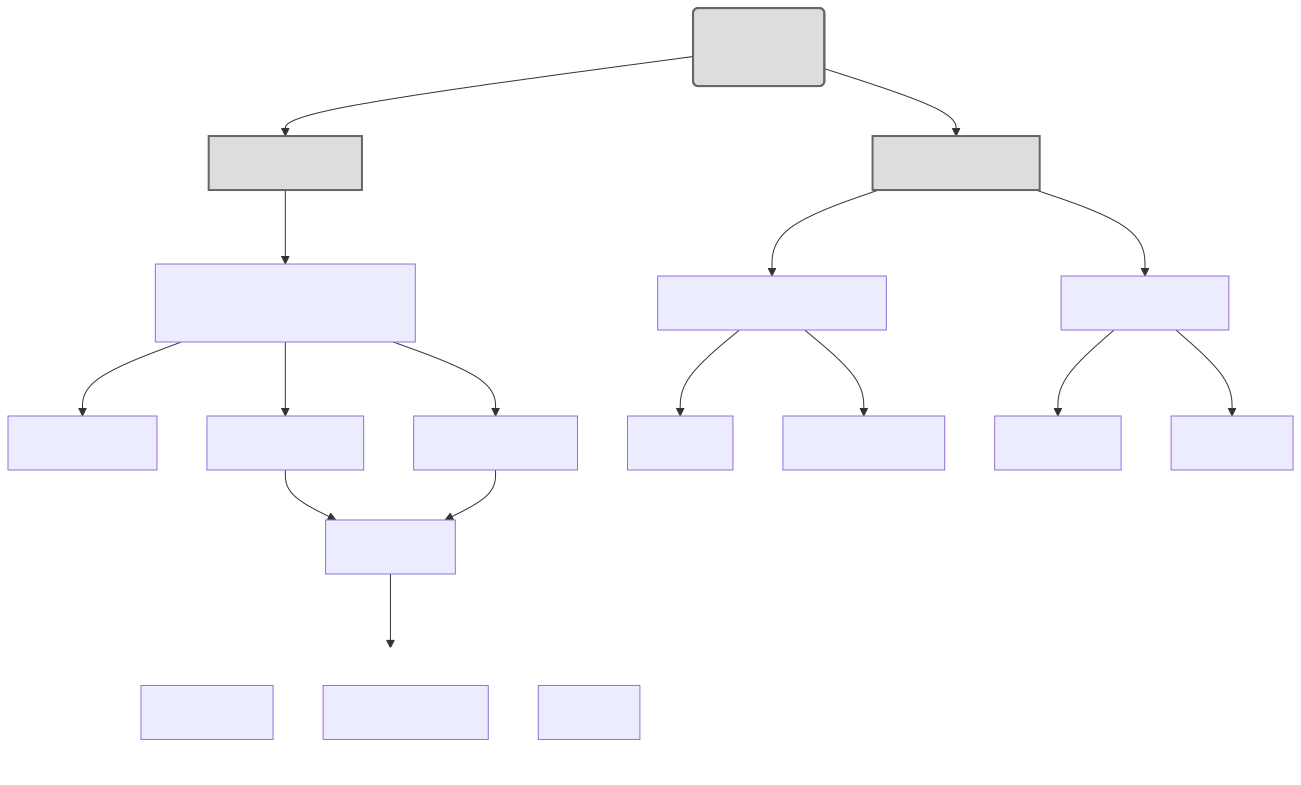
\includegraphics[width=0.9\textwidth]{images/taxonomy-1.png}
    \caption{tassonomia dei attacchi verso modelli di machine learning}
    \label{fig:taxonomy}
\end{figure}


\paragraph{Conoscenza dell'attacante} in base alla conoscenza che l'attaccante possiede del modello di machine learning, gli attacchi possono essere classificati in tre categorie principali:

\begin{itemize}
    \item \textbf{White-box attacks}: L'attaccante ha accesso completo alla struttura del modello, ai parametri, ai pesi, alle funzioni di attivazione e all'algoritmo di training. Questa è la situazione più favorevole per l'attaccante, in quanto può calcolare esattamente come il modello risponde agli input e progettare attacchi altamente efficaci basati su questa conoscenza completa.
    
    \item \textbf{Black-box attacks}: L'attaccante non ha accesso diretto al modello, ma può solo interrogarlo fornendo input e osservando gli output predetti. In questo scenario, l'attaccante deve inferire il comportamento del modello attraverso query ripetute
    
    \item \textbf{Grey-box attacks}: L'attaccante possiede conoscenza parziale del modello. Questo potrebbe includere l'architettura generale del modello, alcuni parametri, informazioni sulla fase di training, oppure accesso a un modello surrogato simile. Questa situazione rappresenta uno scenario intermedio tra gli attacchi white-box e black-box.
\end{itemize}


\paragraph{Specificità dell'attacco}

Se l'obiettivo dell'attaccante è quello che l'esempio generato sia misclassificato in una specifica classe si parla di attacco mirato (\textit{Error-specific attack}) se invece in una classe diversa dall'originale si parla di attacco indiscriminato (\textit{Error-generic})\cite{10.1145/1128817.1128824}

\paragraph{Tempo di attacco}
Un attacco è classificato in base a che fase (training o test) ha come obbiettivo:\cite{10.1145/1128817.1128824}

\begin{itemize}
    \item \textbf{Evasione}: L'avversario può intraprendere un attacco
di evasione contro la classificazione durante la fase di test, producendo
così una percezione errata dal sistema. In questo caso, l'obiettivo dell'avversario
è di ottenere la misclassificazione di alcuni dati per, ad esempio,
rimanere furtivo o mimare un comportamento desiderabile.
    \item \textbf{Poisoning}: L'avversario può avvelenare il dataset di addestramento.
Per ottenere ciò, l'avversario deriva e inietta un punto
per diminuire l'accuratezza della classificazione. Questo attacco ha la
capacità di distorcere completamente la funzione di classificazione durante
il suo addestramento, consentendo così all'attaccante di definire la classificazione
del sistema in qualsiasi modo desideri. L'entità
dell'errore di classificazione dipende dai dati che l'attaccante ha
scelto di avvelenare durante l'addestramento.
\end{itemize} 

\subsection{Manipolazioni comuni che preservano la funzionalità nei file PE}
Considerando la struttura e la funzionalità dei file PE, due manipolazioni basate su byte sono comunemente utilizzate dai attacchi di evasione per preservare sia l' eseguibilità che la funzionalità originale di un file PE. In particolare, le manipolazioni ammissibili basate su byte possono (1) alterare byte in posizioni adatte senza rompere la struttura, oppure (2) iniettare un payload adversarial che non viene mai eseguito. Ad esempio, una manipolazione ammissibile può alterare i primi 58 byte dell'header DOS inutilizzato escludendo le due aree specifiche utilizzate per memorizzare il Magic Number e l'offset al COFF Header\cite{olivander}. Un'altra manipolazione ammissibile può cambiare il nome di ogni sezione modificando le corrispondenti voci della sezione\cite{olivander}. Invece, un payload adversarial può essere aggiunto a un file Windows PE aggiungendo byte di padding alla fine del file binario di input (\textit{padding}), o iniettando una nuova sezione nel file binario accoppiata a una nuova voce di sezione nella Section Table (\textit{section injection}).
Come dimostrato da \cite{10.1145/3473039}, entrambe le operazioni preservano la funzionalità del codice per progettazione, poiché modificano la distribuzione dei byte del codice di input e la struttura del codice ma preservano l'esecuzione del codice. 

Specificamente, la manipolazione \textit{padding} preserva la funzionalità del codice poiché i byte di padding vengono aggiunti alla fine del file binario PE senza introdurre alcuna nuova voce nella Section Table. Di conseguenza, la Section Table continua a mappare dati invariati riguardanti le sezioni del file PE originale. Il file PE rimane eseguibile e il loader del sistema operativo può continuare a caricare le sezioni comuni del file originale. 

\label{secttion_inj}
D'altro canto, la manipolazione \textit{section injection} aggiunge una nuova sezione nell'area Section del file PE. Lo spostamento causato dal codice iniettato introduce un requisito aggiuntivo per preservare la funzionalità del file PE, cioè la necessità di rimappare i riferimenti di memoria delle sezioni originali nella Section Table. Questo viene fatto aggiungendo una voce di 40 byte nella Section Table per specificare informazioni riguardanti la dimensione, l'offset e l'indirizzo di memoria della sezione iniettata. Questa nuova voce richiede il ricalcolo degli offset e degli indirizzi di memoria nelle altre voci della Table Section per mantenere l'allineamento. Anche altre informazioni dell'header (ad es. numero di sezioni, file alignment) vengono aggiornate rispettivamente nel COFF Header e PE Optional Header. Finché gli header e gli allineamenti sono validi, il file binario PE rimane eseguibile. Il payload aggiunto non viene mai eseguito con \textit{padding} o \textit{section injection}. Di conseguenza, entrambe le manipolazioni non alterano il flusso di esecuzione del file originale. 

Tuttavia, la differenza principale tra \textit{padding} e \textit{section injection} è che in \textit{section injection}, l'impronta di memoria (utilizzo della RAM) durante l'esecuzione del codice aumenta poiché la nuova sezione viene carreggiata in memoria anche se mai richiamata per l'esecuzione. Invece, in \textit{padding}, il codice aggiunto non viene caricato in memoria\cite{olivander}.

\subsection{ALgoritmi black-box per la generazione di esempi adversarial per Malware Windows PE}
\subsubsection{GAMMA}

GAMMA (Genetic Adversarial Machine learning Malware Attack)\cite{9437194} è un framework (insieme di algoritmi) per attacchi AML black-box mirati, in accordo con la tassonomia (figura~\ref{fig:taxonomy}) illustrata in precedenza. GAMMA utilizza un algoritmo genetico\cite{deap} per generare esempi adversarial. Risolve un problema di ottimizzazione che massimizza la probabilità di evasione e minimizza la dimensione del contenuto benigno iniettato mediante un termine di penalizzazione che valuta la quantità di contenuto iniettato . Il payload iniettato viene estratto da un insieme di file binari ausiliari (\textit{goodware}), ottimizzandone la selezione e la dimensione tramite operatori di selezione, crossover e mutazione.\cite{9437194}

Oltre alla generazione di payload basandosi su padding o injection, nel framework sono presenti anche altre manipolazioni che preservano la funzionalità, rese disponibili nella libreria secml-malware\cite{demetrio2024secmlmalwarepentestingwindowsmalware}.

\subsubsection{OLIVANDER}

OLIVANDER\cite{olivander} è un metodo adversarial offensivo formulato per attaccare un modello decisionale basato su IA (target model) addestrato per il rilevamento di malware Windows PE dalle feature estratte attraverso l'analisi statica del codice Windows PE eseguita con LIEF.\cite{olivander}

Considerato dunque un modello ML target \(f:LIEF\to \{goodware, malware\}\),
addestrato su un dataset di file PE composto dal feature set descritto in \ref{feature_set}. 
Consideriamo un qualsiasi nuovo malware Windows PE \(x\) correttamente classificato da \(f\) (ossia \(f(LIEF(x))=malware\)).

% OLIVANDER utilizza la conoscenza rivelata dai \textit{counterfactual} (la minima modifica ad \(x\) che altera la predizione di  \(f\)~\cite{evangelatos2025exploringenergylandscapesminimal}) per identificare potenziali vulnerabilità di \(f\) rispetto alla decisione \(f(LIEF(x))\). Sfrutta la conoscenza dei counterfactual per manipolare il codice binario di x e ottenere un malware Windows PE \(x'\) semanticamente invariante, ancora eseguibile, che elude \(f\) (\(f(LIEF(x'))=goodware\)). Come manipolazione del codice, OLIVANDER crea un payload adversarial che viene iniettato in x per ottenere x' attraverso un'operazione di padding o section injection.\cite{olivander}
\paragraph{Funzionamento dell'Algoritmo}
Il metodo OLIVANDER implementa una strategia di evasione \textit{black-box} che sfrutta le spiegazioni \textit{counterfactual} (la minima modifica ad \(x\) che altera la predizione di  \(f\)~\cite{evangelatos2025exploringenergylandscapesminimal})  per guidare la perturbazione del malware. La procedura si articola in tre fasi:

\begin{enumerate}
    \item \textbf{Analisi Statica e Generazione del Target}
     Inizialmente, viene eseguita, mediante la libreria \(LIEF\) un analisi statica di \(x\) per estrarne il vettore delle feature e mappare la distribuzione originale dei byte, definita come \(X_{count}\). Successivamente, viene impiegato il metodo \textit{DiCE-Random} \cite{mothilal2020dice} per generare una spiegazione counterfactual (\(CF\)) limitata alle feature dell'istogramma dei byte. Tale spiegazione agisce come una ``distribuzione target'' ideale, indicando quali valori dell'istogramma dovrebbero essere modificati affinché \(f\) etichetti il campione come benigno, un esempio è fornito in tabella~\ref{tab:esempio_controfattuale}.

    \item \textbf{Ottimizzazione Iterativa della Distribuzione}
    Il nucleo dell'algoritmo è un processo iterativo che lavora su una distribuzione dei byte, denotata come \(X'_{count}\), riferita all'esempio adversarial. Ad ogni iterazione vengono aggiunti ai byte identificati dai CF nel file originale un numero tale di byte tali da avvicinarsi al valore identificato dalla spiegazione CF. Successivamente il valore del byte modificato viene confrontato con il valore suggerito dai CF. Se il valore ottenuto dopo l'aggiunta di byte al file Windows PE è superiore al valore definito dal counterfactual per modificare la predizione, allora viene modificato ulteriormente il file Windows PE andando a decrementare il byte da modificare, cercando di convergere verso il valore suggerito dal CF senza divergere eccessivamente dalla struttura originale.

    \item \textbf{Sintesi del Payload e Verifica dell'Evasione}
Una volta aggiunto il payload al file binario e creato il file avversario questo viene . Questo contenuto viene iniettato nel file binario tramite manipolazioni che preservano la funzionalità (specificamente \textit{padding} o \textit{section injection}) per produrre il candidato avversario \(x'\). Quest'ultimo viene infine sottoposto al modello target \(f\) per verificare l'avvenuta evasione; il ciclo termina se l'attacco ha successo o se viene raggiunto il limite massimo di iterazioni.
\end{enumerate}
\begin{table}[htbp]
    \centering
    \caption{Esempio di spiegazione CF}
    \label{tab:esempio_controfattuale}
    \begin{tabular}{lll}
        \toprule
        Feature istogramma byte & Valore originale & Valore counterfactual \\
        \midrule
        0xA  & 0.00595 & 0.39618 \\
        0x5F & 0.00399 & 0.39499 \\
        \midrule
        \multicolumn{3}{p{0.95\linewidth}}{\small Questo counterfactual spiega che il file malware selezionato potrebbe essere erroneamente classificato come ``goodware'' sostituendo i valori reali (riportati nella colonna 2) delle feature (riportate nella colonna 1) con i corrispondenti valori ``what-if'' (riportati nella colonna 3).tabella recuperata da Olivander\cite{olivander}}. \\
        \bottomrule
    \end{tabular}
\end{table}

Nella creazione di esempi counterfactual, non vengono considerate tutte le feature ma solo le feature riguardi l'istogramma dei byte, poiché è stato osservato\cite{olivander} che questo è il gruppo di feature con \textit{mutual information} (la misura della ``quantità di informazione'' che una variabile casuale contiene riguardo un'altra\cite{mutualInformation_wikipedia}) mediamente più alto.

% \subsubsection{OLIVANDER}

% OLIVANDER è un metodo adversarial offensivo \textit{black-box} progettato per evadere rilevatori di malware Windows PE basati su Intelligenza Artificiale. Il funzionamento del metodo si articola in fasi distinte che collegano lo spazio delle feature (\textit{feature space}) alla manipolazione fisica del file binario (\textit{problem space}).

% \paragraph{Estrazione delle Feature e Analisi Statica}
% Il processo inizia con l'analisi statica del codice binario del malware target \(x\), eseguita mediante la libreria LIEF. Questa fase di parsing trasforma il file eseguibile in una rappresentazione vettoriale composta da 2381 feature statiche grezze~\cite{olivander}. Tale vettore costituisce lo spazio di input per il modello target \(f: \text{LIEF} \to \{\text{goodware, malware}\}\) e aggrega diverse categorie di informazioni, tra cui le \textit{Byte Histogram}, \textit{Byte Entropy Histogram}, informazioni sulle stringhe, sugli header e sulle sezioni.

% \paragraph{Generazione dei Counterfactual}
% Dato un malware \(x\) correttamente classificato da \(f\) (ossia \(f(\text{LIEF}(x)) = \text{malware}\)), OLIVANDER utilizza le tecniche di Explainable AI (XAI) per identificare le vulnerabilità del modello. In particolare, si avvale dei \textit{counterfactual explanations}: spiegazioni di tipo ``what-if'' che indicano la minima perturbazione necessaria al vettore di input affinché la predizione del modello viri dalla classe originale alla classe target (i.e., ``goodware'').
% Per generare queste spiegazioni in uno scenario \textit{black-box} (dove non si ha accesso ai gradienti del modello), OLIVANDER integra il metodo \textit{DiCE-Random}~\cite{olivander}. Questo approccio agisce campionando iterativamente lo spazio di input per trovare una configurazione di feature vicina all'originale ma classificata benigna.

% \paragraph{Manipolazione Guidata dal Feature Space al Problem Space}
% Il contributo distintivo di OLIVANDER risiede nella traduzione delle indicazioni fornite dai counterfactual in modifiche concrete al codice binario. Sebbene LIEF estragga numerose tipologie di feature, il metodo restringe il campo d'azione esclusivamente alle feature del gruppo ``Byte Histogram''. Tale scelta è motivata dall'alta \textit{Mutual Information} osservata tra la distribuzione dei byte e la classificazione del malware, oltre che dalla diretta corrispondenza tra queste feature e il contenuto fisico del file~\cite{olivander}.

% Il meccanismo logico opera come segue:
% \begin{itemize}
%     \item Il counterfactual generato suggerisce quali specifici valori dell'istogramma dei byte devono aumentare affinché il file venga classificato come benigno. Ad esempio, potrebbe indicare che la frequenza del byte \texttt{0xA} deve passare da 0.01 a 0.4.
%     \item OLIVANDER interpreta questa discrepanza come una ``ricetta'' per la costruzione del payload. Il payload adversarial viene riempito esclusivamente con i byte suggeriti dai counterfactual (ossia quei byte il cui conteggio nel file \(x\) è inferiore al valore ``what-if'' proposto dalla spiegazione).
%     \item I byte non indicati dal counterfactual o che non richiedono un incremento vengono ignorati nella costruzione del contenuto aggiuntivo.
% \end{itemize}

% Una volta composto il payload in modo da soddisfare la distribuzione suggerita, esso viene iniettato nel file originale \(x\) tramite operazioni \textit{functionality-preserving} quali \textit{padding} (aggiunta in coda al file) o \textit{section injection} (inserimento di una nuova sezione). Il risultato è un nuovo artefatto \(x'\), semanticamente invariante e ancora eseguibile, il cui vettore di feature \(LIEF(x')\) inganna il classificatore target~\cite{olivander}.
